\chapter{Despliegue y Monitorización}
\label{cap:despliegue}

En el ciclo de vida de la metodología \textbf{Komorebi} \cite{verges_como_2023}, las fases de \textbf{Despliegue de Modelos} e \textbf{Implantación y Monitorización} constituyen el puente indispensable entre los artefactos neuronales validados experimentalmente y su operación continua en un entorno de producción docente. 

Un modelo con altas métricas en laboratorio resulta inútil si no puede integrarse de forma confiable, con tiempos de respuesta viables y una interfaz intuitiva que apoye la labor del evaluador. Para el sistema \textbf{Graphito}, este capítulo documenta la arquitectura de software construida para servir los modelos, la estrategia de persistencia híbrida, la interfaz de usuario en el cliente web y la suite de pruebas y monitorización para garantizar la robustez del sistema.

% ======================================================================
\section{Arquitectura del Backend y Servicios de Inferencia}
\label{sec:arquitectura_backend}
% ======================================================================

El servidor de aplicaciones de Graphito se implementó en Python utilizando el framework \textbf{FastAPI}, ejecutado sobre el servidor ASGI \textbf{Uvicorn}. La elección de FastAPI responde a tres factores técnicos: soporte nativo para programación asíncrona mediante \texttt{async/await}, validación estricta de esquemas de datos en tiempo de ejecución con \textbf{Pydantic} y generación automática de especificaciones OpenAPI (Swagger).

\subsection{Organización por Arquitectura Limpia (\textit{Clean Architecture})}
\label{subsec:clean_architecture}

Para evitar el acoplamiento estrecho entre los frameworks web y los modelos de aprendizaje profundo, el código del backend (directorio \texttt{backend/app/}) se estructuró siguiendo los principios de la Arquitectura Limpia (\textit{Clean Architecture}) formulados por Martin \cite{Martin2017CleanArchitecture}. Bajo este paradigma, las dependencias de software apuntan estrictamente hacia el interior (hacia las reglas de negocio y entidades de dominio), desacoplando los algoritmos de inferencia neuronal y los motores de base de datos de las interfaces de entrega web:

\begin{enumerate}
    \item \textbf{Capa de Dominio (\texttt{domain/}):} Define las entidades fundamentales del sistema académico (\texttt{Submission}, \texttt{Assignment}, \texttt{ReferenceCode}, \texttt{AnalysisReport}) y las reglas de negocio puras, sin dependencias de bases de datos ni bibliotecas externas.
    
    \item \textbf{Capa de Aplicación (\texttt{application/}):} Contiene los casos de uso principales (análisis de entregas, registro de referencias docentes y generación de variantes). Esta capa orquesta el flujo de ejecución: recibe los archivos, invoca el preprocesamiento, solicita la inferencia bimodal y persiste el reporte.
    
    \item \textbf{Capa de Infraestructura (\texttt{infrastructure/}):} Provee las implementaciones técnicas concretas. Aloja los adaptadores de persistencia (SQLAlchemy para PostgreSQL y ChromaDB para vectores) y los motores de inferencia (\textit{GraphCodeBERT}, \textit{CharCNN} y \textit{BimodalFusion}).
    
    \item \textbf{Capa de Presentación (\texttt{presentation/}):} Expone los controladores y rutas REST estructurados en módulos de API (autenticación, gestión de asignaciones y análisis bimodal). Maneja la serialización de respuestas y la captura de errores HTTP estandarizados.
\end{enumerate}

\subsection{Pipeline de Inferencia Asíncrono}
\label{subsec:pipeline_inferencia_backend}

Para dar cumplimiento al requerimiento de tiempo de respuesta (RNF-01: procesamiento menor a 20 segundos por entrega), la inferencia bimodal se ejecuta de forma concurrente:

\begin{itemize}
    \item Al recibir una solicitud en el endpoint \texttt{POST /api/v1/analysis/evaluate}, el servidor valida la extensión del archivo (\texttt{.c} o \texttt{.cpp}) y dispara dos tareas concurrentes en un hilo de trabajo asíncrono (\texttt{asyncio.gather}):
    \begin{enumerate}
        \item Extracción de AST y DFG mediante Tree-sitter y cálculo del vector de atención lógica en GraphCodeBERT con LoRA.
        \item Extracción de la secuencia de caracteres crudos normalizados y cálculo de la probabilidad sintética $p_{\text{IA}}$ con MultiScaleCharCNN.
    \end{enumerate}
    \item Las salidas se combinan en memoria mediante \texttt{BimodalFusion}, comparando el vector resultante contra la colección de soluciones de referencia indexadas para la asignación correspondiente.
\end{itemize}

% ======================================================================
\section{Capa de Persistencia Híbrida: Relacional y Vectorial}
\label{sec:persistencia_hibrida}
% ======================================================================

Graphito requiere gestionar simultáneamente dos naturalezas de información cualitativamente distintas: datos transaccionales estructurados (cuentas docentes, materias, catálogos de problemas, metadatos de auditoría) y tensores densos de alta dimensionalidad correspondientes a las firmas semánticas y estilométricas.

Para resolver esta dualidad, se implementó un esquema de \textbf{persistencia híbrida}, dividiendo la responsabilidad en dos motores especializados:

\subsection{Base de Datos Relacional: PostgreSQL}
\label{subsec:db_postgresql}

La gestión transaccional se apoya en \textbf{PostgreSQL} a través del ORM \textbf{SQLAlchemy} y la herramienta de migraciones \textbf{Alembic}. Los modelos relacionales (definidos en el módulo de base de datos de infraestructura, archivo \texttt{models.py}) aseguran la integridad referencial y las reglas de privacidad docente (RN-02):

\begin{itemize}
    \item \textbf{Usuarios y Roles:} Cuentas de profesores con contraseñas cifradas mediante algoritmo Argon2/Bcrypt y tokens JWT para autorización.
    \item \textbf{Asignaciones y Grupos:} Estructura organizativa de cursos, ligando cada problema algorítmico a sus especificaciones técnicas y soluciones de referencia autorizadas.
    \item \textbf{Historial de Evaluaciones:} Registro inmutable de cada análisis procesado, almacenando fecha, identificador anonimizado de la entrega, similitud lógica obtenida, probabilidad de IA calculada, dictamen emitido y observaciones ingresadas por el docente.
\end{itemize}

\subsection{Base de Datos Vectorial: ChromaDB}
\label{subsec:db_chromadb}

Para las representaciones neuronales densas, se utiliza \textbf{ChromaDB} como motor de almacenamiento vectorial. Las ventajas de esta integración comprenden:

\begin{itemize}
    \item \textbf{Indexación HNSW:} ChromaDB implementa el algoritmo de grafos jerárquicos de pequeños mundos navegables (\textit{Hierarchical Navigable Small World}, HNSW), desarrollado por Malkov y Yashunin \cite{Malkov2020HNSW}. Esta estructura de indexación en grafos multidimensionales permite resolver búsquedas aproximadas de vecinos más cercanos ($k$-NN) sobre el vector unificado de 1792 dimensiones con complejidad logarítmica $\mathcal{O}(\log N)$, logrando tiempos de respuesta inferiores a $15\,\text{ms}$ incluso con colecciones de referencia densas.
    \item \textbf{Espacio de Distancia Coseno:} La colección se inicializa con la métrica de similitud del coseno:
    \begin{equation}
        d_{\text{cos}}(u, v) = 1 - \frac{u \cdot v}{\|u\| \|v\|}
    \end{equation}
    permitiendo contrastar instantáneamente el código del alumno contra todas las variantes de referencia del ejercicio sin necesidad de recomputar los embeddings de los códigos base.
\end{itemize}

En la Tabla~\ref{tab:persistencia_hibrida} se sintetizan las responsabilidades, tecnologías y métricas operativas de ambos motores en el esquema de persistencia híbrida.

\begin{table}[H]
    \centering
    \caption{Comparativa técnica de persistencia híbrida: PostgreSQL vs ChromaDB.}
    \label{tab:persistencia_hibrida}
    \renewcommand{\arraystretch}{1.25}
    \small
    \begin{tabularx}{\textwidth}{|l|X|X|}
        \hline
        \textbf{Criterio de Diseño} & \textbf{Motor Relacional (PostgreSQL)} & \textbf{Motor Vectorial (ChromaDB)} \\ \hline
        Naturaleza de los Datos & Estructurados, relacionales y transaccionales (cumplimiento ACID). & Vectores densos de alta dimensión ($v_{\text{fused}} \in \mathbb{R}^{1792}$) y metadatos. \\ \hline
        Entidades Gestionadas & Docentes, asignaciones, ejercicios, bitácora de auditoría y roles. & Embeddings de soluciones de referencia y variantes sintéticas. \\ \hline
        Mecanismo de Acceso & Consultas declarativas SQL mediante ORM SQLAlchemy y migraciones Alembic. & Búsqueda aproximada de vecinos más cercanos ($k$-NN) vía API en Python. \\ \hline
        Estructura de Indexación & Índices de árbol B-Tree en llaves primarias y restricciones foráneas. & Grafo jerárquico de pequeños mundos navegables (HNSW \cite{Malkov2020HNSW}). \\ \hline
        Métrica de Consulta & Coincidencia exacta, operadores lógicos y filtros relacionales. & Distancia de Coseno angular ($d_{\text{cos}} \in [0, 2]$). \\ \hline
        Complejidad Temporal & $\mathcal{O}(1)$ por clave primaria; $\mathcal{O}(\log N)$ en búsquedas indexadas. & $\mathcal{O}(\log N)$ para consultas de similitud aproximada de vecinos. \\ \hline
        Latencia Operativa & $< 5\,\text{ms}$ en consultas transaccionales típicas. & $< 15\,\text{ms}$ en cálculo de proximidad sobre colecciones densas. \\ \hline
    \end{tabularx}
\end{table}

% ======================================================================
\section{Capa de Presentación e Interfaz de Usuario}
\label{sec:interfaz_usuario}
% ======================================================================

La interfaz de usuario de Graphito se diseñó siguiendo los principios de la arquitectura modular y centrada en el usuario (\textit{User-Centered Design}). Se implementó como una aplicación de página única (\textit{Single Page Application}) construida con \textbf{React 18}, \textbf{TypeScript}, el framework utilitario \textbf{Tailwind CSS} y empaquetada mediante \textbf{Vite}.

\subsection{Componentes Principales de la Plataforma}
\label{subsec:componentes_ui}

La plataforma web (directorio \texttt{frontend/}) organiza las interacciones del profesor en tres módulos clave:

\subsubsection{Biblioteca de Referencias y Asignaciones}
El panel principal permite al docente explorar sus grupos activos, dar de alta nuevos ejercicios algorítmicos y gestionar las soluciones oficiales de referencia. En la Figura~\ref{fig:ui_biblioteca} se muestra la vista de la biblioteca.

\begin{figure}[H]
    \centering
    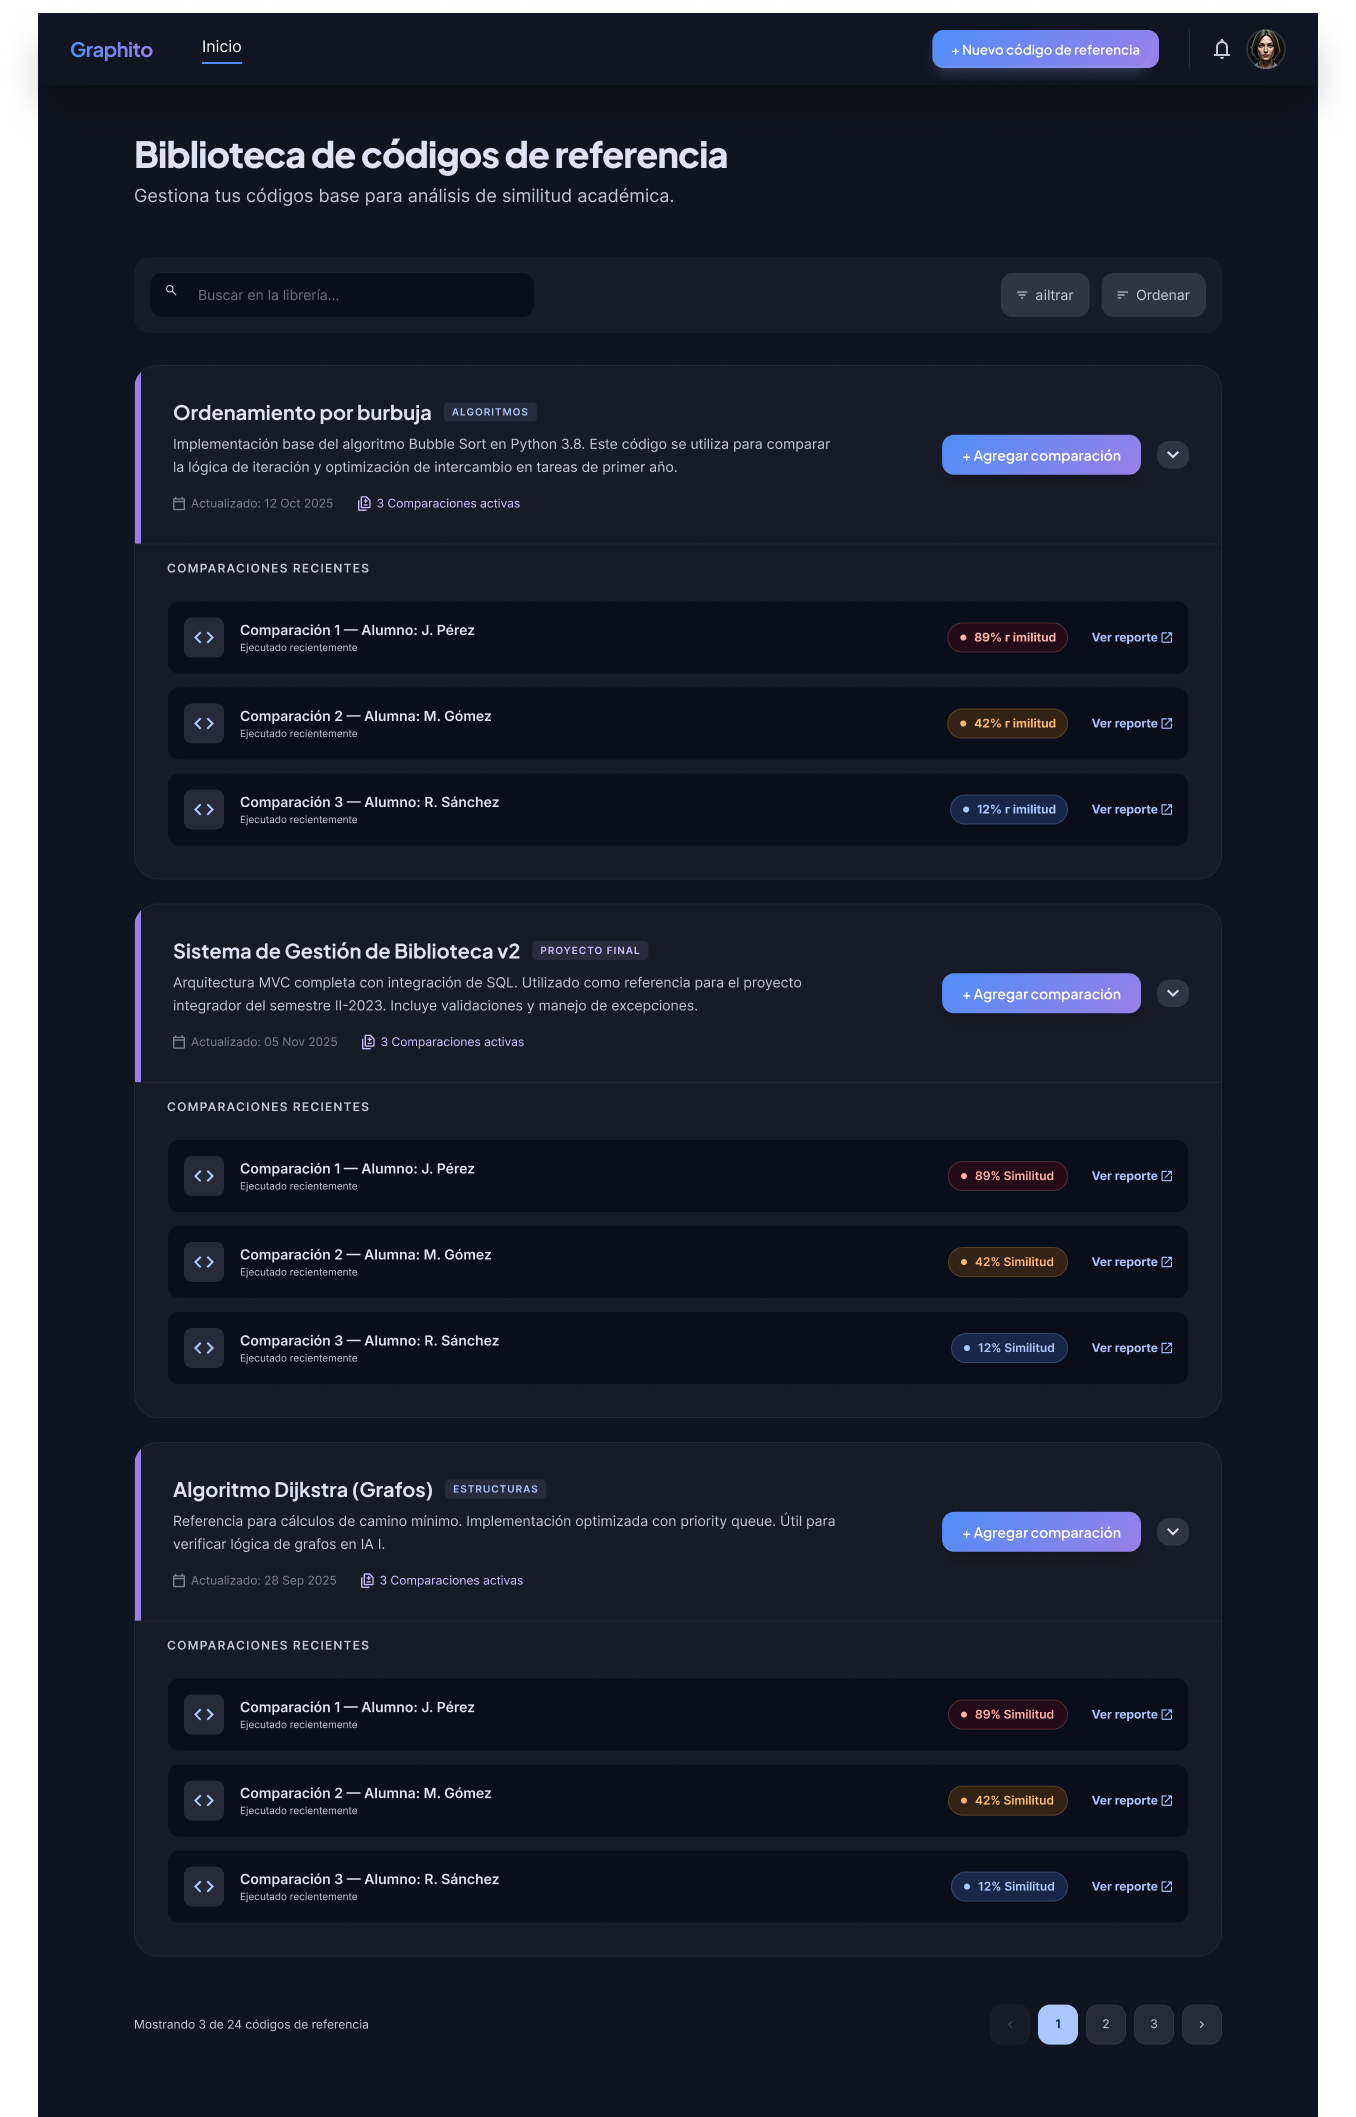
\includegraphics[width=0.88\textwidth]{figuras/biblioteca_de_referencias.png}
    \caption{Módulo de biblioteca de referencias y gestión de asignaciones docentes.}
    \label{fig:ui_biblioteca}
\end{figure}

\subsubsection{Carga y Parametrización de Soluciones}
Permite cargar el código fuente de referencia en C o C++, asociarle su enunciado algorítmico y activar la generación de variantes sintéticas controladas mediante LLMs locales o externos. En la Figura~\ref{fig:ui_nueva_referencia} se ilustra el modal de carga.

\begin{figure}[H]
    \centering
    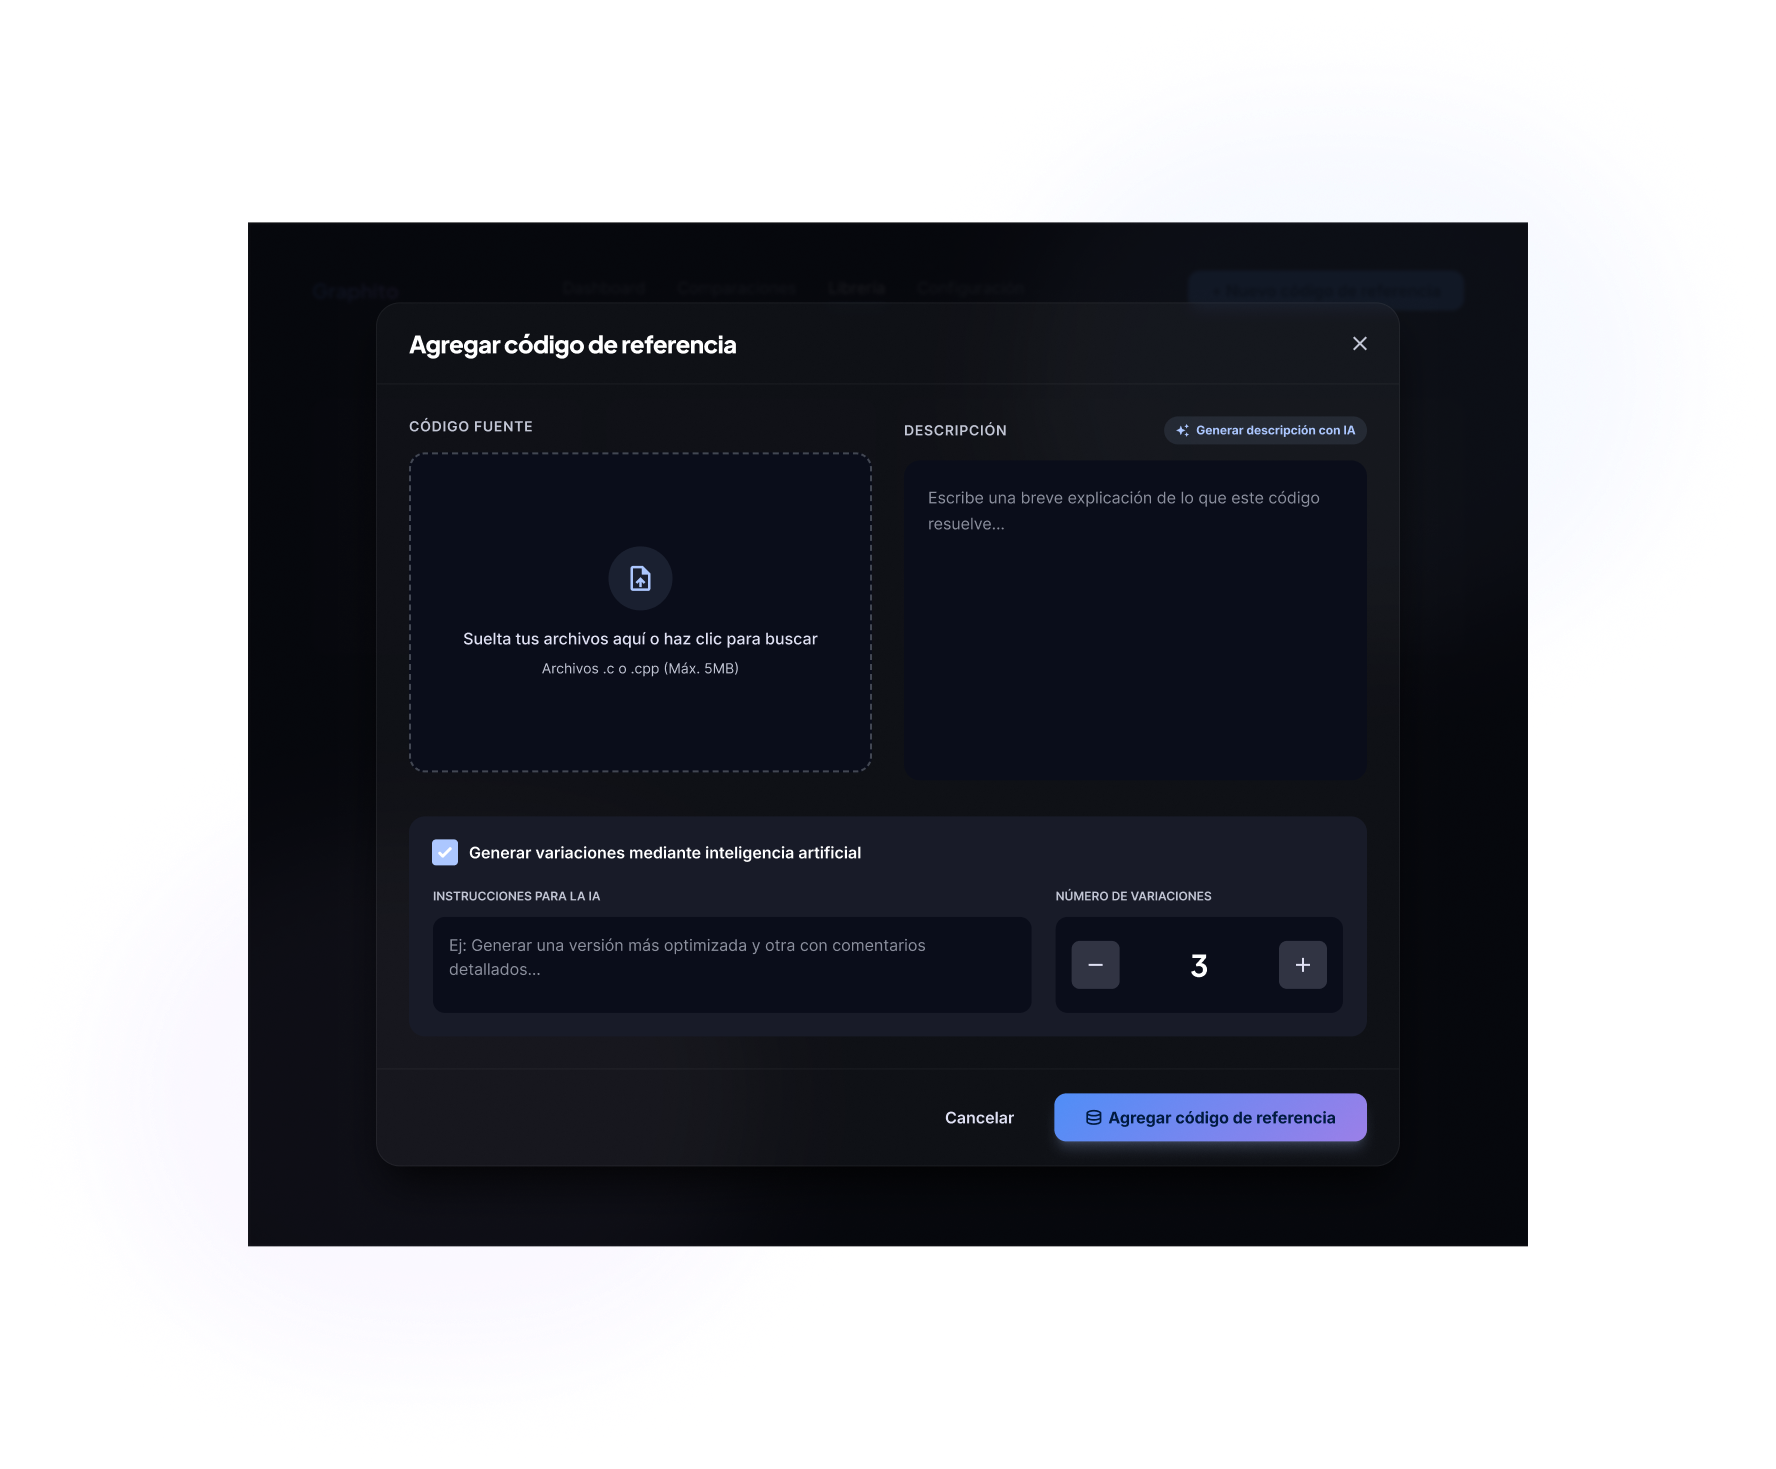
\includegraphics[width=0.85\textwidth]{figuras/nuevo_código_de_referencia.png}
    \caption{Interfaz para la carga y parametrización de nuevas soluciones de referencia.}
    \label{fig:ui_nueva_referencia}
\end{figure}

\subsubsection{Panel de Reporte de Similitud e Integridad}
En cumplimiento estricto con la regla de negocio \textbf{RN-04} y los principios de explicabilidad en el despliegue de modelos de aprendizaje automático formulados por Bhatt et al. \cite{Bhatt2020Explainable}, el sistema adopta un diseño centrado en el humano (\textit{Human-in-the-Loop}). Graphito nunca emite sanciones automáticas ni califica al alumno de forma autónoma. En su lugar, el reporte visualiza de manera desagregada e interpretable los dos indicadores (gráfico de similitud lógica y probabilidad estilométrica), brindando al docente una herramienta de soporte a la decisión fundamentada técnicamente para guiar la entrevista presencial de evaluación. En la Figura~\ref{fig:ui_reporte_similitud} se muestra el panel interactivo del reporte.

\begin{figure}[H]
    \centering
    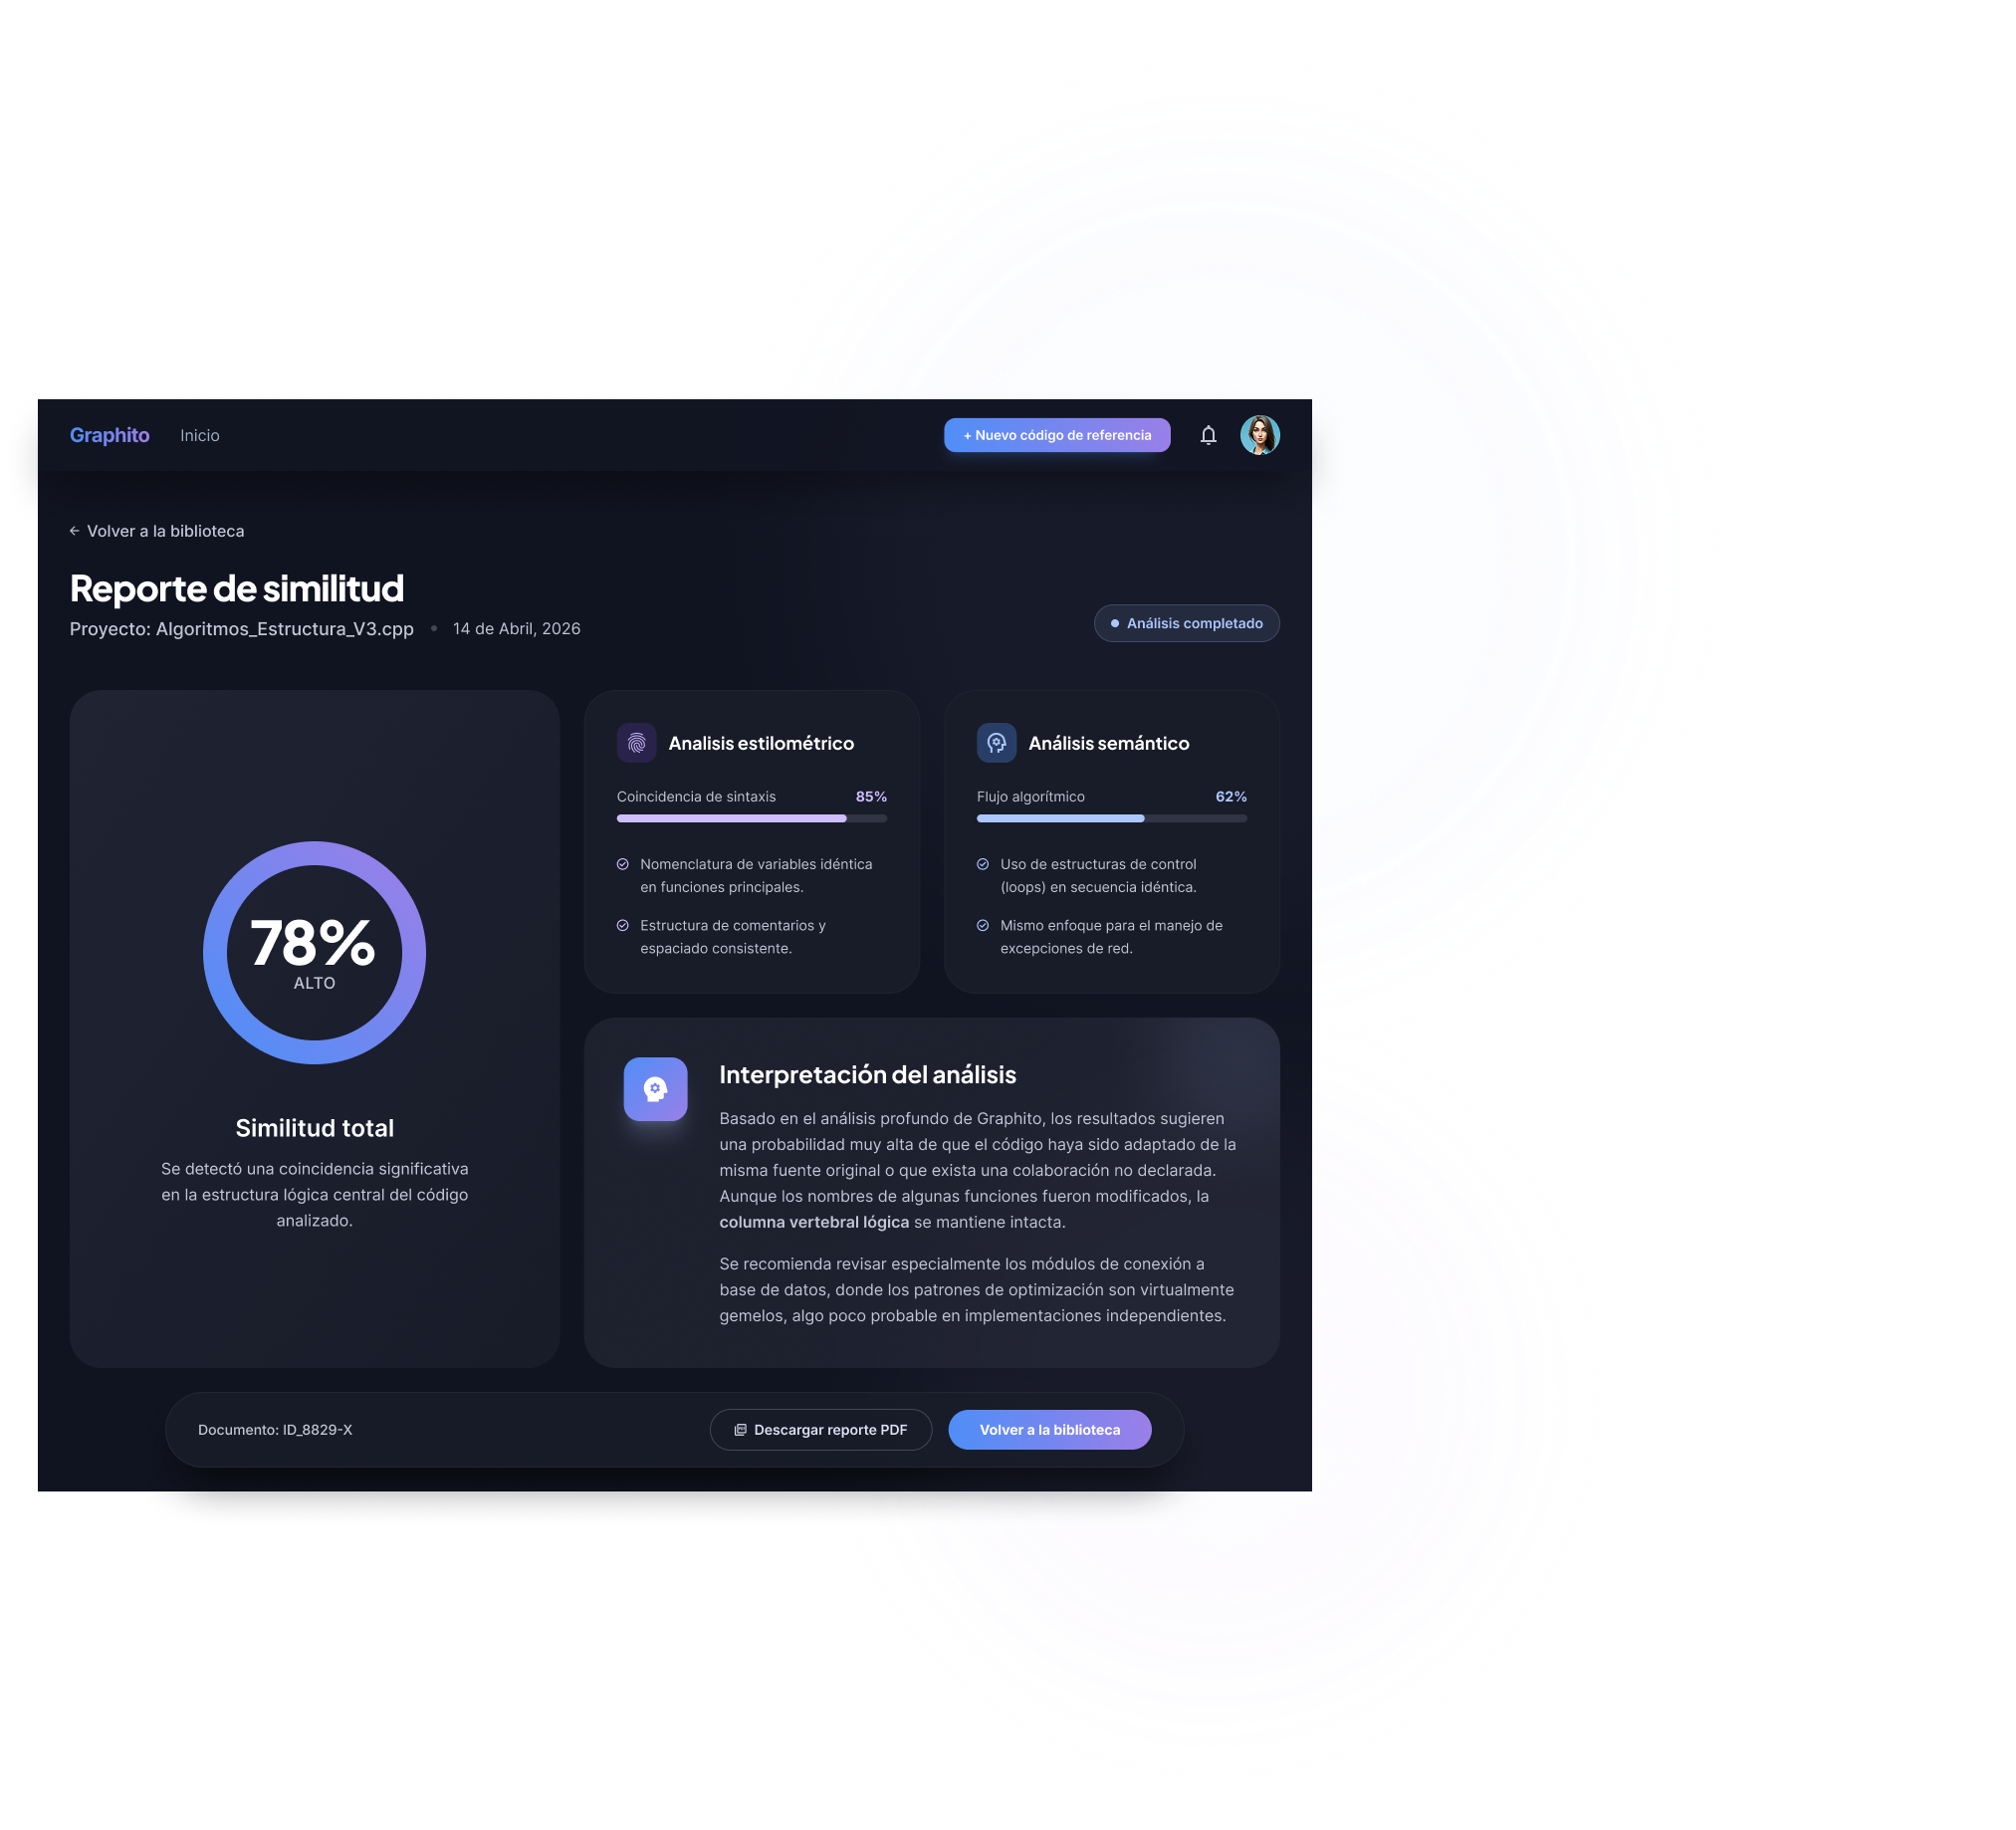
\includegraphics[width=0.88\textwidth]{figuras/reporte_de_similitud.png}
    \caption{Panel interactivo del reporte de integridad académica con indicadores bimodales.}
    \label{fig:ui_reporte_similitud}
\end{figure}

% ======================================================================
\section{Infraestructura y Despliegue de la Solución}
\label{sec:infraestructura_despliegue}
% ======================================================================

Para que el sistema funcione en la práctica y pueda ser utilizado por los profesores sin complicaciones, no basta con tener los programas desarrollados en una computadora; es necesario distribuirlos en internet de manera confiable, segura y económica. 

En lugar de montar todo el sistema en una sola máquina (lo que provocaría lentitud o caídas si el equipo se satura o se apaga), se diseñó una estrategia distribuida en la que cada parte de la plataforma se ubica en el lugar más adecuado según su función:

\begin{figure}[H]
    \centering
    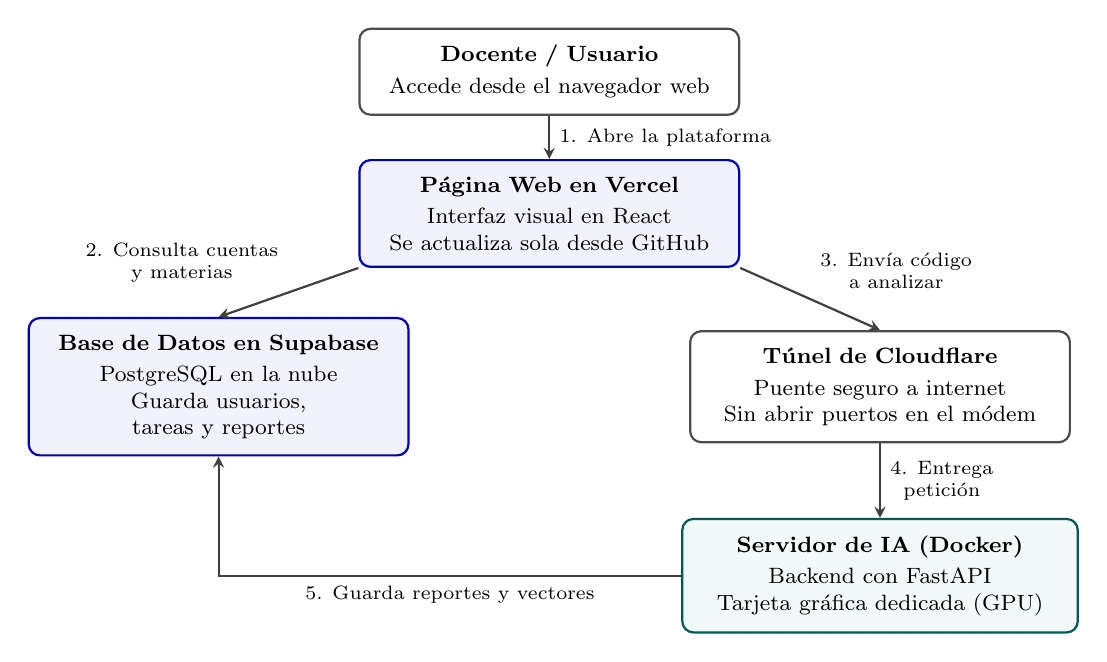
\begin{tikzpicture}[
        box/.style={
            rectangle, 
            rounded corners=4pt, 
            draw=black!70, 
            thick, 
            fill=white, 
            text width=4.4cm, 
            align=center, 
            inner sep=6pt, 
            font=\footnotesize
        },
        cloudbox/.style={
            rectangle, 
            rounded corners=4pt, 
            draw=blue!70!black, 
            thick, 
            fill=blue!5, 
            text width=4.4cm, 
            align=center, 
            inner sep=6pt, 
            font=\footnotesize
        },
        localbox/.style={
            rectangle, 
            rounded corners=4pt, 
            draw=teal!70!black, 
            thick, 
            fill=teal!5, 
            text width=4.6cm, 
            align=center, 
            inner sep=6pt, 
            font=\footnotesize
        },
        arrow/.style={->, >=stealth, thick, draw=black!75}
    ]
    % Nodos con coordenadas fijas
    \node[box] (docente) at (0, 0) {\textbf{Docente / Usuario}\\[2pt]Accede desde el navegador web};
    \node[cloudbox] (vercel) at (0, -1.8) {\textbf{Página Web en Vercel}\\[2pt]Interfaz visual en React\\Se actualiza sola desde GitHub};
    
    \node[cloudbox] (supabase) at (-4.2, -4.0) {\textbf{Base de Datos en Supabase}\\[2pt]PostgreSQL en la nube\\Guarda usuarios, tareas y reportes};
    \node[box] (cloudflare) at (4.2, -4.0) {\textbf{Túnel de Cloudflare}\\[2pt]Puente seguro a internet\\Sin abrir puertos en el módem};
    
    \node[localbox] (docker) at (4.2, -6.4) {\textbf{Servidor de IA (Docker)}\\[2pt]Backend con FastAPI\\Tarjeta gráfica dedicada (GPU)};
    
    % Conexiones
    \draw[arrow] (docente) -- node[right, font=\scriptsize]{1. Abre la plataforma} (vercel);
    \draw[arrow] (vercel.south west) -- node[above left, font=\scriptsize, align=center]{2. Consulta cuentas\\y materias} (supabase.north);
    \draw[arrow] (vercel.south east) -- node[above right, font=\scriptsize, align=center]{3. Envía código\\a analizar} (cloudflare.north);
    \draw[arrow] (cloudflare) -- node[right, font=\scriptsize, align=center]{4. Entrega\\petición} (docker);
    \draw[arrow] (docker.west) -| node[pos=0.25, below, font=\scriptsize]{5. Guarda reportes y vectores} (supabase.south);
    \end{tikzpicture}
    \caption{Distribución física de los servicios y flujo de comunicación del sistema Graphito.}
    \label{fig:arquitectura_despliegue}
\end{figure}

A continuación se detalla cómo opera cada una de estas piezas y la razón práctica por la que se configuraron de esta manera:

\subsection{Interfaz Web en Vercel y Actualización Automática desde GitHub}
\label{subsec:despliegue_frontend}

La pantalla que ven y utilizan los profesores (el \textit{frontend}) no se hospeda en una computadora personal ni en un servidor escolar, sino en \textbf{Vercel}, una plataforma en la nube especializada en servir aplicaciones web a escala global. 

Una ventaja fundamental de este enfoque es su conexión directa con el repositorio del proyecto en \textbf{GitHub}. Cada vez que el equipo de desarrollo realiza una mejora en el diseño, corrige un botón o agrega una nueva función y guarda los cambios en GitHub, Vercel detecta la actualización automáticamente, reconstruye la página y la pone en línea en cuestión de dos minutos. De esta forma, el docente siempre cuenta con la versión más reciente del sistema sin necesidad de reinstalar nada ni sufrir cortes en el servicio.

\subsection{Base de Datos en Supabase (PostgreSQL en la Nube)}
\label{subsec:despliegue_supabase}

Para que la información de los profesores, sus grupos, las tareas y los reportes generados estén siempre seguros y disponibles, se utilizó \textbf{Supabase}, un servicio que provee una base de datos PostgreSQL hospedada en la nube. 

Tener la base de datos en la nube evita depender del almacenamiento de la computadora local. Si por alguna razón la máquina física donde se analizan los modelos se apaga o se desconecta temporalmente, la información de los usuarios y el historial de evaluaciones pasadas continúan intactos y pueden consultarse desde cualquier dispositivo con internet. Además, este servicio realiza copias de seguridad continuas para prevenir la pérdida de información.

\subsection{Servidor de Inteligencia Artificial en Equipo Local con Tarjeta Gráfica (GPU)}
\label{subsec:despliegue_gpu}

Los dos modelos de inteligencia artificial que dan vida a Graphito (GraphCodeBERT y MultiScaleCharCNN) requieren analizar simultáneamente la lógica y los caracteres de cada programa entregado. Este proceso involucra millones de operaciones matemáticas matriciales. 

Si estos cálculos se realizaran con el procesador convencional (CPU) de una computadora normal, el análisis de un solo código podría tardar varios minutos, lo cual resultaría impráctico en una clase con decenas de estudiantes. Por esta razón, el backend del sistema se instaló en una computadora equipada con una \textbf{tarjeta gráfica dedicada (GPU)}. Las tarjetas gráficas están especialmente diseñadas para realizar miles de operaciones matemáticas al mismo tiempo (cálculo en paralelo), permitiendo que el análisis completo tome menos de 10 segundos.

Asimismo, emplear un equipo propio con GPU evita los altos costos mensuales que implicaría alquilar servidores de inteligencia artificial con tarjeta gráfica en proveedores comerciales de la nube, haciendo que el proyecto sea completamente viable y sostenible para el entorno académico.

\subsection{Empaquetamiento en Contenedores con Docker}
\label{subsec:despliegue_docker}

En el desarrollo de software suele ocurrir un problema común: un programa funciona perfectamente en la computadora de quien lo creó, pero falla al intentar instalarlo en otra máquina debido a diferencias en el sistema operativo, versiones distintas de librerías o controladores incompatibles.

Para resolver este reto de raíz y prevenir lo que Sculley et al. \cite{Sculley2015TechnicalDebt} señalan como la acumulación de deuda técnica oculta y fragilidad de dependencias en sistemas de aprendizaje automático, el servidor de Graphito se empaquetó utilizando \textbf{Docker}. Un contenedor Docker opera como una ``caja virtual'' sellada y reproducible que guarda el programa junto con todo lo que necesita para ejecutarse: la versión exacta de Python, las librerías de análisis de código (Tree-sitter, Clang-Format) y los paquetes de inteligencia artificial (PyTorch y CUDA). Gracias a esto, el sistema se enciende con un solo comando y funciona de manera idéntica y reproducible en cualquier equipo compatible.

\subsection{Conexión Segura hacia Internet mediante un Túnel de Cloudflare}
\label{subsec:despliegue_cloudflare}

Dado que la computadora con la tarjeta gráfica se encuentra dentro de una red local privada (como la red de un laboratorio o un domicilio) y no cuenta con una dirección IP pública fija en internet, la página web alojada en Vercel no tendría forma de comunicarse con ella para enviarle los códigos a revisar.

La solución tradicional para este problema solía ser ``abrir puertos'' en el módem de internet. Sin embargo, abrir puertos es una práctica muy riesgosa porque deja una puerta abierta para que personas no autorizadas o programas maliciosos intenten atacar la red interna.

Para resolver este dilema de forma segura, se utilizó un \textbf{Túnel de Cloudflare} mediante la utilidad \texttt{cloudflared}. En lugar de abrir la red local hacia afuera, el túnel establece una conexión saliente segura y cifrada desde el equipo hacia los servidores de Cloudflare en internet. Cuando un profesor sube un archivo en la página web, la petición viaja protegida y llega directamente a la tarjeta gráfica de la máquina local. Este mecanismo protege la red contra accesos no autorizados, garantiza que la comunicación cuente con un certificado digital seguro (HTTPS) y evita configuraciones complejas en el módem.

% ======================================================================
\section{Pruebas, Verificación y Monitorización del Sistema}
\label{sec:pruebas_monitorizacion}
% ======================================================================

La última fase de la metodología Komorebi corresponde a la \textbf{Monitorización y Cierre}, asegurando que el sistema mantenga su confiabilidad operativa y detecte degradaciones o derivas de datos (*data drift*).

\subsection{Suite de Pruebas Automatizadas con Pytest}
\label{subsec:pruebas_pytest}

Para garantizar la robustez, mantenibilidad y estabilidad operativa del sistema ante actualizaciones continuas de dependencias o nuevos modelos, en el directorio \texttt{tests/} se estructuró una suite exhaustiva de pruebas automatizadas ejecutadas bajo el framework \textbf{Pytest}. En la Tabla~\ref{tab:pruebas_automatizadas_pytest} se detallan los módulos de prueba implementados, los componentes evaluados, los escenarios cubiertos y sus respectivos criterios de aceptación.

\begin{table}[htbp]
    \centering
    \caption{Estructura y cobertura de la suite de pruebas automatizadas en Pytest.}
    \label{tab:pruebas_automatizadas_pytest}
    \renewcommand{\arraystretch}{1.25}
    \small
    \begin{tabularx}{\textwidth}{|>{\raggedright\arraybackslash}p{3.3cm}|X|X|>{\raggedright\arraybackslash}p{3.1cm}|}
        \hline
        \textbf{Módulo de Prueba} & \textbf{Componente Auditado} & \textbf{Escenarios y Validaciones} & \textbf{Criterio de Aceptación} \\ \hline
        \texttt{test\_}\allowbreak\texttt{dfg\_}\allowbreak\texttt{parser.py} & Parser sintáctico (Tree-sitter C/C++) & Punteros dobles, estructuras anidadas, macros de preprocesador y operadores unarios. & Construcción de DFG sin excepciones y grafo consistente. \\ \hline
        \texttt{test\_}\allowbreak\texttt{char\_cnn\_}\allowbreak\texttt{robustness.py} & Invarianza estilométrica de MultiScaleCharCNN & Variaciones de sangría, código con y sin comentarios, reordenamiento cosmético. & Desviación en probabilidad $|\Delta p_{\text{IA}}| \le 0.05$. \\ \hline
        \texttt{test\_}\allowbreak\texttt{e2e\_}\allowbreak\texttt{analysis.py} & Pipeline completo de inferencia y API REST & Flujo extremo a extremo: recepción HTTP, inferencia dual paralela y persistencia. & Tiempo de respuesta total $< 5.0\,\text{s}$ en entorno local. \\ \hline
        \texttt{test\_}\allowbreak\texttt{calibration\_}\allowbreak\texttt{experiment.py} & Calibración del umbral operativo ($\tau$) & Barrido de umbrales sobre muestras de validación y simulación de corte. & Tasa de falsos positivos $\text{FPR} < 10.0$\,\% (cumple RNF-06). \\ \hline
    \end{tabularx}
\end{table}

La ejecución automatizada de esta suite en el entorno de desarrollo y pruebas asegura la detección temprana de regresiones funcionales antes de realizar cualquier despliegue hacia el servidor de producción.

\subsection{Estrategia de Monitorización y Mitigación de Falsos Positivos}
\label{subsec:estrategia_monitorizacion}

Para evitar decisiones arbitrarias o sesgadas durante la implantación del sistema en materias de programación, se definieron tres salvaguardas operativas de monitorización:

\begin{enumerate}
    \item \textbf{Bitácora de Auditoría Inmutable (\textit{Audit Log}):} Siguiendo las directrices de mitigación de deuda técnica en sistemas de aprendizaje automático de Sculley et al. \cite{Sculley2015TechnicalDebt}, cada análisis registra de forma inmutable las trazas intermedias de inferencia ($v_{\text{sem}}$, $p_{\text{IA}}$, versión del checkpoint cargado y marcas de tiempo). Ante cualquier aclaración solicitada por un estudiante, el docente dispone de evidencia auditable y reproducible que sustenta técnicamente la evaluación.
    \item \textbf{Mecanismo de Re-calibración y Adaptación ante Deriva:} La evolución acelerada de las herramientas generativas comerciales induce el fenómeno de deriva de datos y conceptos (\textit{concept drift}), formalizado por Gama et al. \cite{Gama2014ConceptDrift}. Para evitar la degradación progresiva en la discriminación estilométrica, se contempla un protocolo de reentrenamiento periódico incorporando muestras sintéticas actualizadas generadas con \texttt{generar\_referencias.py}.
    \item \textbf{Diseño de Soporte a la Decisión (\textit{Human-in-the-Loop}):} Con base en los principios éticos y operativos de explicabilidad formulados por Bhatt et al. \cite{Bhatt2020Explainable}, el sistema opera estrictamente como un apoyo analítico para el docente y nunca como un juez automático, preservando en todo momento el juicio pedagógico y los derechos académicos del estudiantado.
\end{enumerate}

% ======================================================================
\section{Conclusión del capítulo}
\label{sec:conclusion_despliegue}
% ======================================================================

La culminación de las fases de Despliegue y Monitorización de la metodología Komorebi consolida a Graphito como una plataforma integral de ingeniería de software. La estructuración en Clean Architecture sobre FastAPI, la persistencia dual en PostgreSQL y ChromaDB, la interfaz orientada a la experiencia docente en React y la rigurosa suite de pruebas automatizadas garantizan que los modelos de inteligencia artificial operen con eficiencia, seguridad y pleno apego a los principios de integridad pedagógica. Con esto, el sistema se encuentra preparado para su validación formal y cierre metodológico.
